\begin{wrapfigure}[8]{r}{0pt}
	\begin{tikzpicture}[scale=4]
\draw[thick, ->] (-0.2, 0) -- (1, 0);
\draw[thick, ->] (0, -0.5) -- (0, 1);
\draw[red, domain=0.005:1, samples=1500] plot(\x, {\x * sin((1/\x) r)}) node [above right] {$x\cdot \sin(\frac{1}{x})$};
\draw[blue, thin] (0, 0) -- (0.7, 0.7);
\draw[blue, thin] (0, 0) -- (0.7, -0.7);
\end{tikzpicture}
\end{wrapfigure}

\paragraph{Exemple}

\[\begin{array}{rcl}
f:&[0, +\infty[ & \rightarrow \mathbb{R} \\
&x& \mapsto \left\{\begin{array}{rl}
	x\sin(\frac{1}{x}) & \text{si } x \neq 0 \\
	0 & \text{ si } x = 0
\end{array}
\right.
\end{array}\]

On remarque que f(0) n'est ni un minimum, ni un maximum local.

\section{Acroissements finis et conséquences}


\paragraph{Exemple}

\begin{wrapfigure}[4]{l}{0pt}
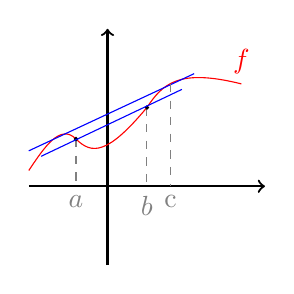
\begin{tikzpicture}
\draw[thick, ->] (-1, 0) -- (2, 0);
\draw[thick, ->] (0, -1) -- (0, 2);
\draw[red] (-1, 0.2) .. controls (-0.8, 0.5) and (-0.6, 0.8) .. (-0.4, 0.6);
\draw[red] (-0.4, 0.6) .. controls (-0.2, 0.4) and (0, 0.4) .. (0.5, 1);
\draw[red] (0.5, 1) .. controls (0.7, 1.3) and (0.9, 1.5) .. (1.7, 1.3) node [right, above] {$f$};

\draw[gray, dashed] (-0.4, 0.6) -- (-0.4, 0) node [below] {$a$};
\draw[gray, dashed] (0.5, 1) -- (0.5, 0) node [below] {$b$};

\draw[fill=black] (-0.4, 0.6) circle (0.02) coordinate (A);
\draw[fill=black] (0.5, 1) circle (0.02) coordinate (B);

\draw[blue] (-0.844, 0.38)  -- (0.944, 1.23);
\draw[blue] (-1, 0.45)  -- (1.1, 1.43);
\draw[gray, dashed] (0.8, 1.3) -- (0.8, 0) node [below] {c};

\end{tikzpicture}
\end{wrapfigure}

\paragraph{Théorème} $f:[a, b] \rightarrow \mathbb{R}$ est continue sur $[a, b]$ et dérivable sur $]a, b[$.
Il existe un réel $c \in ]a, b[$ tel que $\frac{f(b)-f(a)}{b-a} = f'(c)$.

\paragraph{Démonstration} Appliquer le théorème de Rolle à  ~\\
$g(x) = f(x) - (\frac{f(b)-f(a)}{b-a})\cdot x$

\paragraph{Corollaire} f est une fonction comme ci dessus, 

\begin{itemize}
\item si $f' \geq 0$ sur $]a, b[$ alors f est croissante sur $[a, b]$
\item si $f' > 0$ sur $]a, b[$ alors f est strictement croissante sur $[a, b]$
\item si $f' \leq 0$ sur $]a, b[$ alors f est decroissante sur $[a, b]$
\item si $f' < 0$ sur $]a, b[$ alors f est strictement decroissante sur $[a, b]$
\item si $f' = 0$ sur $]a, b[$ alors f est constante $[a, b]$
\end{itemize}

\paragraph{Application} Tableaux de variations.

\paragraph{Exemple} \[
\begin{array}{rcl}
\sin h :& \mathbb{R} \rightarrow \mathbb{R} \\
&x& \mapsto \frac{e^x - e^{-x}}{2}
\end{array}\]

$\sin h (0) = 0$ $\sin h$ est dérivable sur $\mathbb{R}$ et $\sin h'(x) = \frac{e^x + e^-x}{2} = cos h(x)$ ~\\
$sinh'(x) > 0$ pour tout x, donc le sinus hyperbolique est croissante.

De même \[ 
\begin{array}{rcl}
\cos h :& \mathbb{R} \rightarrow \mathbb{R} \\
&x& \mapsto \frac{e^x + e^{-x}}{2}
\end{array}\]

$\cos 'h(x) = \frac{e^x + e^{-x}}{2}' = \frac{e^x - e^{-x}}{2} = \sin h$
~\\ $\cos(0) = 1$


\begin{tikzpicture}
	\tkzTab[espcl=6]{$x$/1,$sin'h$/1,$sinh$/2}{$-\infty$, $+\infty$}{,+}{-/$-\infty$,+/$+\infty$}
	\tkzTabVal[draw]{1}{2}{0.5}{$0$}{$0$}
\end{tikzpicture}

\begin{tikzpicture}
	\tkzTab{$x$/1,$cos'h$/1,$cosh$/2}{$-\infty$, $0$, $+\infty$}{,-,z,+}{+/$+\infty$,-/$1$,+/$+\infty$}
\end{tikzpicture}


\[ 
\begin{array}{rcl}
\tan h :& \mathbb{R} \rightarrow &\mathbb{R} \\
&x \mapsto & \frac{sinh(x)}{cosh(x)} = \frac{e^x - e^{-x}}{e^x + e^{-x}}
\end{array}\]

\[\begin{array}{rcl}
\frac{e^x - e^{-x}}{e^x + e^{-x}} &=& \frac{e^x(1-e^{-2x})}{e^x(1+e^{-2x})} \\
														  &=& \frac{1-e^{-2x}}{1+e^{-2x}} \xrightarrow[x \to +\infty]{} 1

\end{array}\]

De la même façon, $tan h(x) \xrightarrow[x \to -\infty]{} = -1$

% Faire le sinus, cosinus et tangeante hyperbolique graphiquement

\paragraph{Remarque} $\sin h : \mathbb{R} \rightarrow \mathbb{R}$ est bijective $\sin h^{-1} = arg \sin h$~\\
$\cos h : \mathbb{R}^+ \rightarrow [1, +\infty[$ est bijective $\cos h^{-1} = arg \cos h$

\chapter{Dérivées d'ordre supérieur}

\paragraph{But} Approcher localement une fonction f par des polynômes.
\paragraph{Définition} $\begin{array}{rl}
	k \in \mathbb{N}^+,& k!=1*2*3*...*k \\
						&0! = 1 \end{array}$
\paragraph{Exemple}
\begin{itemize}
	\item $\begin{array}{rcl}
			\text{ polynome de degré 0 } f(x) &=& f(x_0)+(f(x)-f(x_0)) \\
&=& \epsilon (x) \xrightarrow[x \to x_0]{} 0 \text { Si f continue}\end{array}$
		\item Polynôme de degré 1 si f est dérivable : ~\\
			$\begin{array}{rcl}
				f(x) &=& f(x_0) + f'(x_0)(x-x_0)+(f(x)-f(x_0)-f'(x_0)(x-x_0)) \\
						 (f(x)-f(x_0)-f'(x_0)(x-x_0)) &=& (x-x_0)(\frac{f(x)-f(x_0)}{x-x_0} - f'(x_0))\\
																																	&=& \epsilon (x) \xrightarrow[x \to x_0]{} 0 \text{ car f est dérivable}
			\end{array}$

On voudrait ~\\
	$f(x) = f(x_0)+f'(x_0)(x-x_0) + \frac{1}{2!}f''(x_0)(x-x_0)^2 + \frac{1}{3!}f^{(3)}(x_0)(x-x_0)^3 + ...+ \frac{1}{n!}f^{(n)}(x_0)(x-x_0)^n+(x-x_0)^n \epsilon(x)$ ~\\
avec $\epsilon (x) \xrightarrow[x\to x_0]{} 0$
\end{itemize}


Objectifs du cours : 
\begin{enumerate}
	\item Comprendre $f''(x_0), f'''(x_0)$
	\item Comprendre $\epsilon (x)$
\end{enumerate}

\newpage
\begin{wrapfigure}[7]{r}{0pt}
\begin{tikzpicture}
	\clip (-1, -1) -- (5, -1) -- (5, 5) -- (-1, 5) -- cycle;
	\draw[->] (-1, 0) -- (3, 0);
	\draw[->] (0, -1) -- (0, 3);
	\draw[red, domain=-1:3] plot(\x, {exp(\x)}) node [right] {$y=e^x$};
	\draw[blue, domain=-1:3] plot(\x, {\x + 1}) node [right] {$y=1+x$};
\end{tikzpicture}
\end{wrapfigure}


\paragraph{Exemple} En $0$ ordre 2 : $e^x = 1+x+\frac{1}{2}x^2+x^2\epsilon (x)$ ~\\
Application : 
\begin{itemize}
	\item Calcul de limites : $\frac{e^x-1-x}{x^2} \xrightarrow[x \to 0]{} \frac{1}{2}$
	\item Position d'un graph par rapport à sa tangeante. On considère $f(x) - \text{ tangeante }$: \[\begin{array}{rcl}
		e^x - (x-1) &=& \frac{1}{2}x^2 + x^2 \epsilon(x) \\
											   &=& x^2(\frac{1}{2}+\epsilon(x))
\end{array}\]
\end{itemize}

$x^2 > 0$ et $\frac{1}{2} + \epsilon (x) > 0$ donc près de 0, la fonction est au dessus de sa tangeante.

\section{Dérivées d'ordre supérieur}

\paragraph{Définition} $f : I \rightarrow \mathbb{R}$ I est un intervalle ouvert.
On dit que f est $C^0$ si elle est : 
\begin{itemize}
	\item $C^0$ si elle est continue sur I.
	\item $C^1$ si elle est dérivable sur I \ul{et} que f' est continue.
	\item $C^2$ si f est dérivable deux fois et f'' est continue sur I
	\item $C^k$ si f est dérivable k fois et $f^{(k)}$ est continue sur I
	\item $C^\infty$ si f est $C^k \forall k \in \mathbb{N}$
\end{itemize}

\paragraph{Exemple}

$f(x)=x^2\sin(\frac{1}{x}) \rightarrow C^0$ car $f(x)$ est dérivable, donc continue.
\[\begin{array}{rcl}
		f'(x) &=& 2x \sin(\frac{1}{x})+x^2(\frac{-1}{x^2})\cos(\frac{1}{x}) \\
					   &=& 2x\sin(\frac{1}{x}) - \cos\frac{1}{x}
\end{array}\]

Donc $f(x)$ n'est pas $C^1$ car $f'(x)$ n'est pas continue ($\cos(\frac{1}{x})$ n'est pas continue en 0).

\section{Développement limité et formule de Taylor-Young}

\paragraph{Définition} Soit $f : I \rightarrow \mathbb{R}$, I est un intervalle ouvert. $x_0 \in I$.
f admet un développement limité en $x_0$ à l'ordre n s'il existe : 
\begin{itemize}
	\item un polynome de degrés n : $P(x) = a_0+a_1.x+...+a_n.x^n$
	\item Un fonction $\epsilon : ]x_0-\delta, x_0+\delta[ \rightarrow \mathbb{R}$ avec $\epsilon \xrightarrow[x \to x_0]{} 0$ tel que  \[ \begin{array}{rcl}
			f(x) &=& P(x-x_0)+(x-x_0).\epsilon(x) \text{ pour } x \in ]x_0-\delta, x_0+\delta[ \\
					   &=& a_0+a_1(x-x_0)+...+a_n(x-x_n)^n\epsilon(x) 
	\end{array}\]

	Dans ce cas P est la partie principale du développement limité.
\end{itemize}
